% Digital Logic Report Template
% Created: 2020-01-10, John Miller

%==========================================================
%=========== Document Setup  ==============================

% Formatting defined by class file
\documentclass[11pt]{article}

% ---- Document formatting ----
\usepackage[margin=1in]{geometry}	% Narrower margins
\usepackage{booktabs}				% Nice formatting of tables
\usepackage{graphicx}				% Ability to include graphics

%\setlength\parindent{0pt}	% Do not indent first line of paragraphs 
\usepackage[parfill]{parskip}		% Line space b/w paragraphs
%	parfill option prevents last line of pgrph from being fully justified

% Parskip package adds too much space around titles, fix with this
\RequirePackage{titlesec}
\titlespacing\section{0pt}{8pt plus 4pt minus 2pt}{3pt plus 2pt minus 2pt}
\titlespacing\subsection{0pt}{4pt plus 4pt minus 2pt}{-2pt plus 2pt minus 2pt}
\titlespacing\subsubsection{0pt}{2pt plus 4pt minus 2pt}{-6pt plus 2pt minus 2pt}

% ---- Hyperlinks ----
\usepackage[colorlinks=true,urlcolor=blue]{hyperref}	% For URL's. Automatically links internal references.

% ---- Code listings ----
\usepackage{listings} 					% Nice code layout and inclusion
\usepackage[usenames,dvipsnames]{xcolor}	% Colors (needs to be defined before using colors)

% Define custom colors for listings
\definecolor{listinggray}{gray}{0.98}		% Listings background color
\definecolor{rulegray}{gray}{0.7}			% Listings rule/frame color

% Style for Verilog
\lstdefinestyle{Verilog}{
	language=Verilog,					% Verilog
	backgroundcolor=\color{listinggray},	% light gray background
	rulecolor=\color{blue}, 			% blue frame lines
	frame=tb,							% lines above & below
	linewidth=\columnwidth, 			% set line width
	basicstyle=\small\ttfamily,	% basic font style that is used for the code	
	breaklines=true, 					% allow breaking across columns/pages
	tabsize=3,							% set tab size
	commentstyle=\color{gray},	% comments in italic 
	stringstyle=\upshape,				% strings are printed in normal font
	showspaces=false,					% don't underscore spaces
}

% How to use: \Verilog[listing_options]{file}
\newcommand{\Verilog}[2][]{%
	\lstinputlisting[style=Verilog,#1]{#2}
}




%======================================================
%=========== Body  ====================================
\begin{document}

\title{ELC 2137 Lab 05: Intro to Verilog}
\author{Kyra Rose}

\maketitle


\section*{Summary}

In this lab, we are introduced to coding verilog in Vivado. We built the three circuits, half adder, full adder, and 2 bit adder, in Vivado and observed their behavioral simulations. After viewing their simulations, I can conclude that the results were as I expected in my truth table. 


\section*{Q\&A}

What is one thing that you still don't understand about Verilog?

I still don't understand what exactly a test bench is a how to make an instance. 

\section*{Code}

\begin{lstlisting}[style=Verilog,
	caption=Half Adder code,
	label=code:ex 
	]
	module halfadder(
	input a,
	input b,
	output c,
	output s
	);
	
	assign c=a&b;
	assign s=a^b;
	endmodule
	
	module halfadder_test();
	reg a;
	reg b;
	wire c;
	wire s;
	
	halfadder dut(
	.a(a),
	.b(b),
	.c(c),
	.s(s)
	);
	
	initial begin
	a=0;b=0;#10;
	a=0;b=1;#10;
	a=1;b=0;#10;
	a=1;b=1;#10;
	$finish;
	end 
\end{lstlisting}

\begin{lstlisting}[style=Verilog,
	caption=Full Adder code,
	label=code:ex 
	]
	module fulladder(
	input cin,
	input ain,
	input bin,
	output cout,
	output sout
	);
	
	wire c1;
	wire c2;
	wire s1;
	
	halfadder ha0 (
	.a(ain),
	.b(bin),
	.c(c1),
	.s(s1)
	);
	
	halfadder ha1 (
	.a(ain),
	.b(bin),
	.c(c2),
	.s(sout)
	);
	
	assign cout= c1 | c2;
	
	endmodule
	
	module fulladder_test();
	
	reg cin;
	reg a;
	reg b;
	wire cout;
	wire s;
	
	fulladder dut(
	.cin(cin),
	.ain(a),
	.bin(b),
	.cout(cout),
	.sout(s)
	);
	
	initial begin
	cin=0; a=0; b=0; #10;
	cin=0; a=0; b=1; #10;
	cin=0; a=1; b=0; #10;
	cin=0; a=1; b=1; #10;
	cin=1; a=0; b=0; #10;
	cin=1; a=0; b=1; #10;
	cin=1; a=1; b=0; #10;
	cin=1; a=1; b=1; #10;
	
	$finish;
	end
\end{lstlisting}

\begin{lstlisting}[style=Verilog,
	caption=Adder Subtractor code,
	label=code:ex 
	]
module addsub(
input [1:0] a,
input [1:0] b,
input mode,
output [1:0] sum,
output cbout
);

wire c1;
wire c2;
wire [1:0] b_n;
wire y1;
wire y0;
wire cout;

assign b_n = ~b;
assign y0 = b_n[0] ^ mode;
assign y1 = b_n[1] ^ mode;

fulladder fa0 (
.cin(mode),
.ain(a[0]),
.bin(y0),
.cout(c1),
.sout(sum[0])
);

fulladder fa1 (
.cin(mode),
.ain(a[1]),
.bin (y1),
.cout(cbout),
.sout(sum[1])
);

assign cbout = mode ^ cout; 


endmodule

module addsub_test();

reg [1:0] a;
reg [1:0] b;
reg mode;
wire [1:0] sum;
wire cbout;

addsub dut(
.a(a),
.b(b),
.mode(mode),
.sum(sum),
.cbout(cbout)
);

initial begin

a=2'b00; b=2'b01; mode=0; #10; mode=1; #10;
a=2'b00; b=2'b10; mode=0; #10; mode=1; #10;
a=2'b00; b=2'b11; mode=0; #10; mode=1; #10;
a=2'b01; b=2'b01; mode=0; #10; mode=1; #10;
a=2'b10; b=2'b01; mode=0; #10; mode=1; #10;
a=2'b10; b=2'b00; mode=0; #10; mode=1; #10;

$finish;
end

endmodule

\end{lstlisting}


\section*{Results}

\begin{table}[h]\centering
	\caption{Half Adder Truth Table }
	\label{tbl:example_table}
	\begin{tabular}{cc|cc}
		\toprule
		A & B & C & S \\
		\midrule
		0 & 0 & 0 & 0 \\
		0 & 1 & 0 & 1 \\
		1 & 0 & 0 & 1 \\
		1 & 1 & 1 & 0 \\
		\bottomrule
	\end{tabular} 
\end{table}

\begin{figure}[h]\centering
	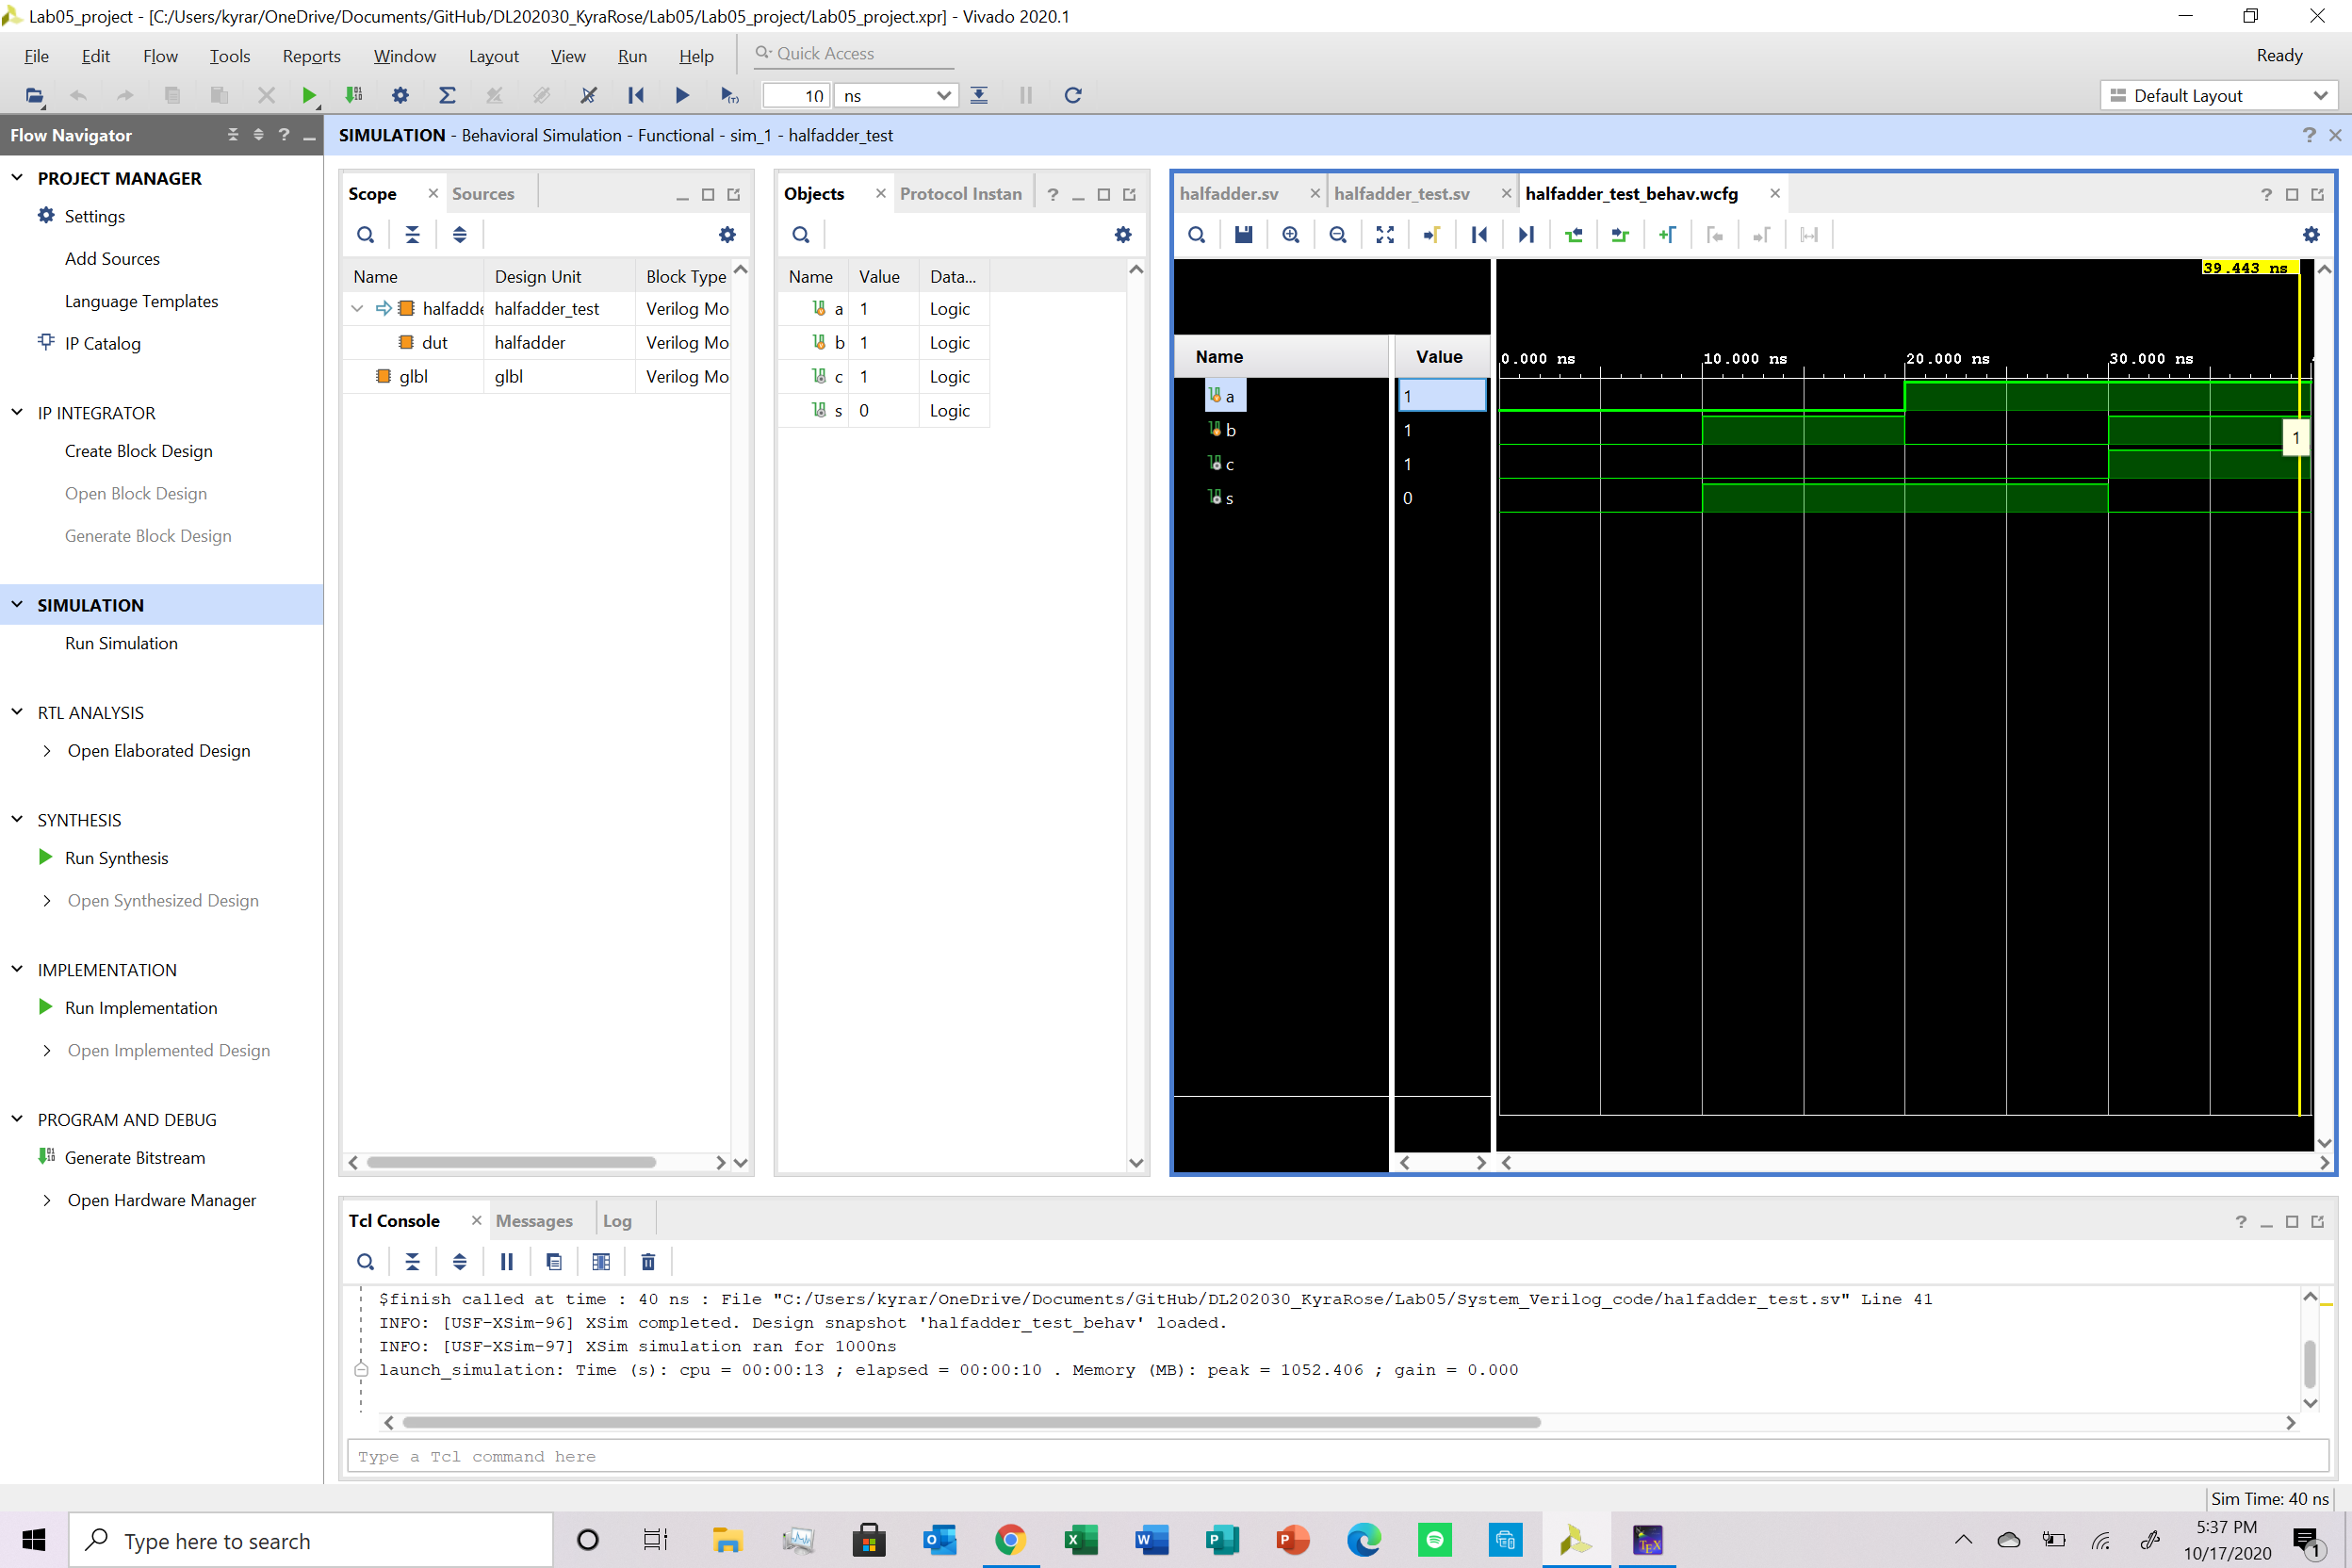
\includegraphics[width=0.5\textwidth,trim=43cm 30cm 0cm 8cm,clip]{halfadder sim}
	\caption{Half Adder Behavioral Simulation}
\end{figure}

\begin{figure}[h]\centering
	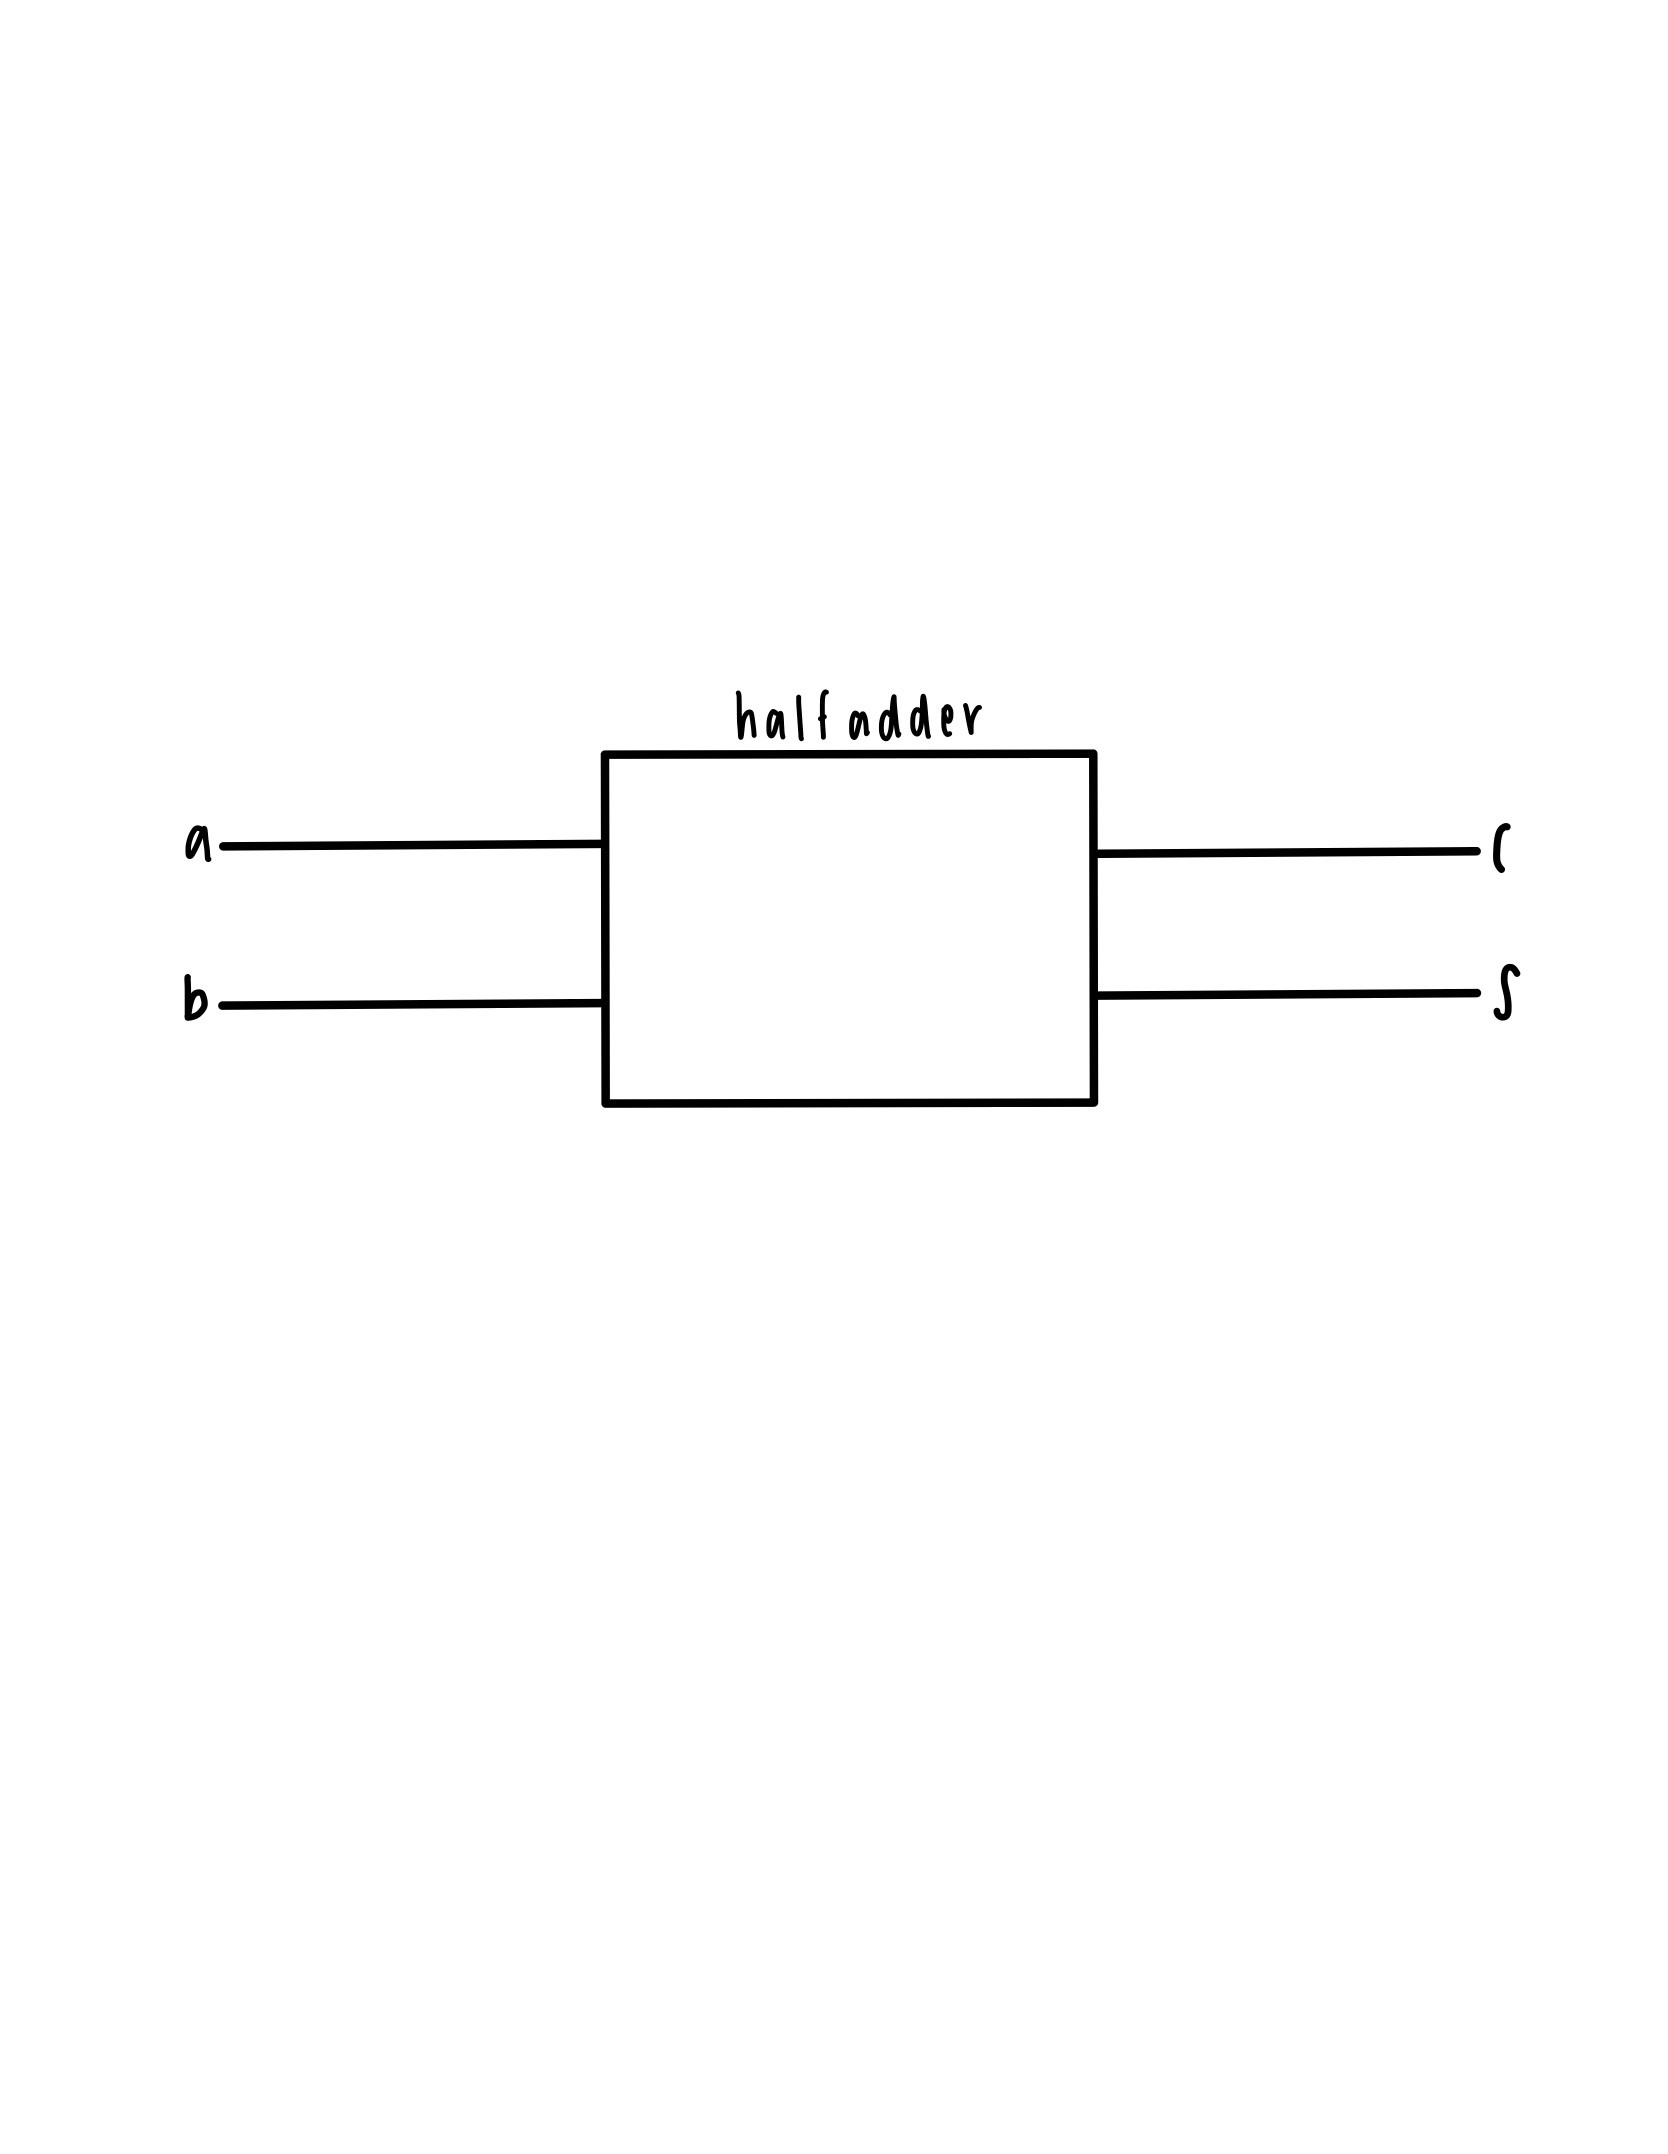
\includegraphics[width=0.5\textwidth,trim=0cm 25cm 0cm 15cm,clip]{halfadder block diagram}
	\caption{Half Adder Block Diagram}
\end{figure}

\begin{table}[h]\centering
	\caption{Full Adder Truth Table }
	\label{tbl:example_table}
	\begin{tabular}{ccc|cc}
		\toprule
		Cin & A & B & Cout & S \\
		\midrule
		0 & 0 & 0 & 0 & 0 \\
		0 & 0 & 1 & 0 & 1 \\
		0 & 1 & 0 & 0 & 1 \\
		0 & 1 & 1 & 1 & 0 \\
		1 & 0 & 0 & 0 & 1 \\
		1 & 0 & 1 & 1 & 0 \\
		1 & 1 & 0 & 1 & 0 \\
		1 & 1 & 1 & 1 & 1 \\
		\bottomrule
	\end{tabular} 
\end{table}

\begin{figure}[h]\centering
	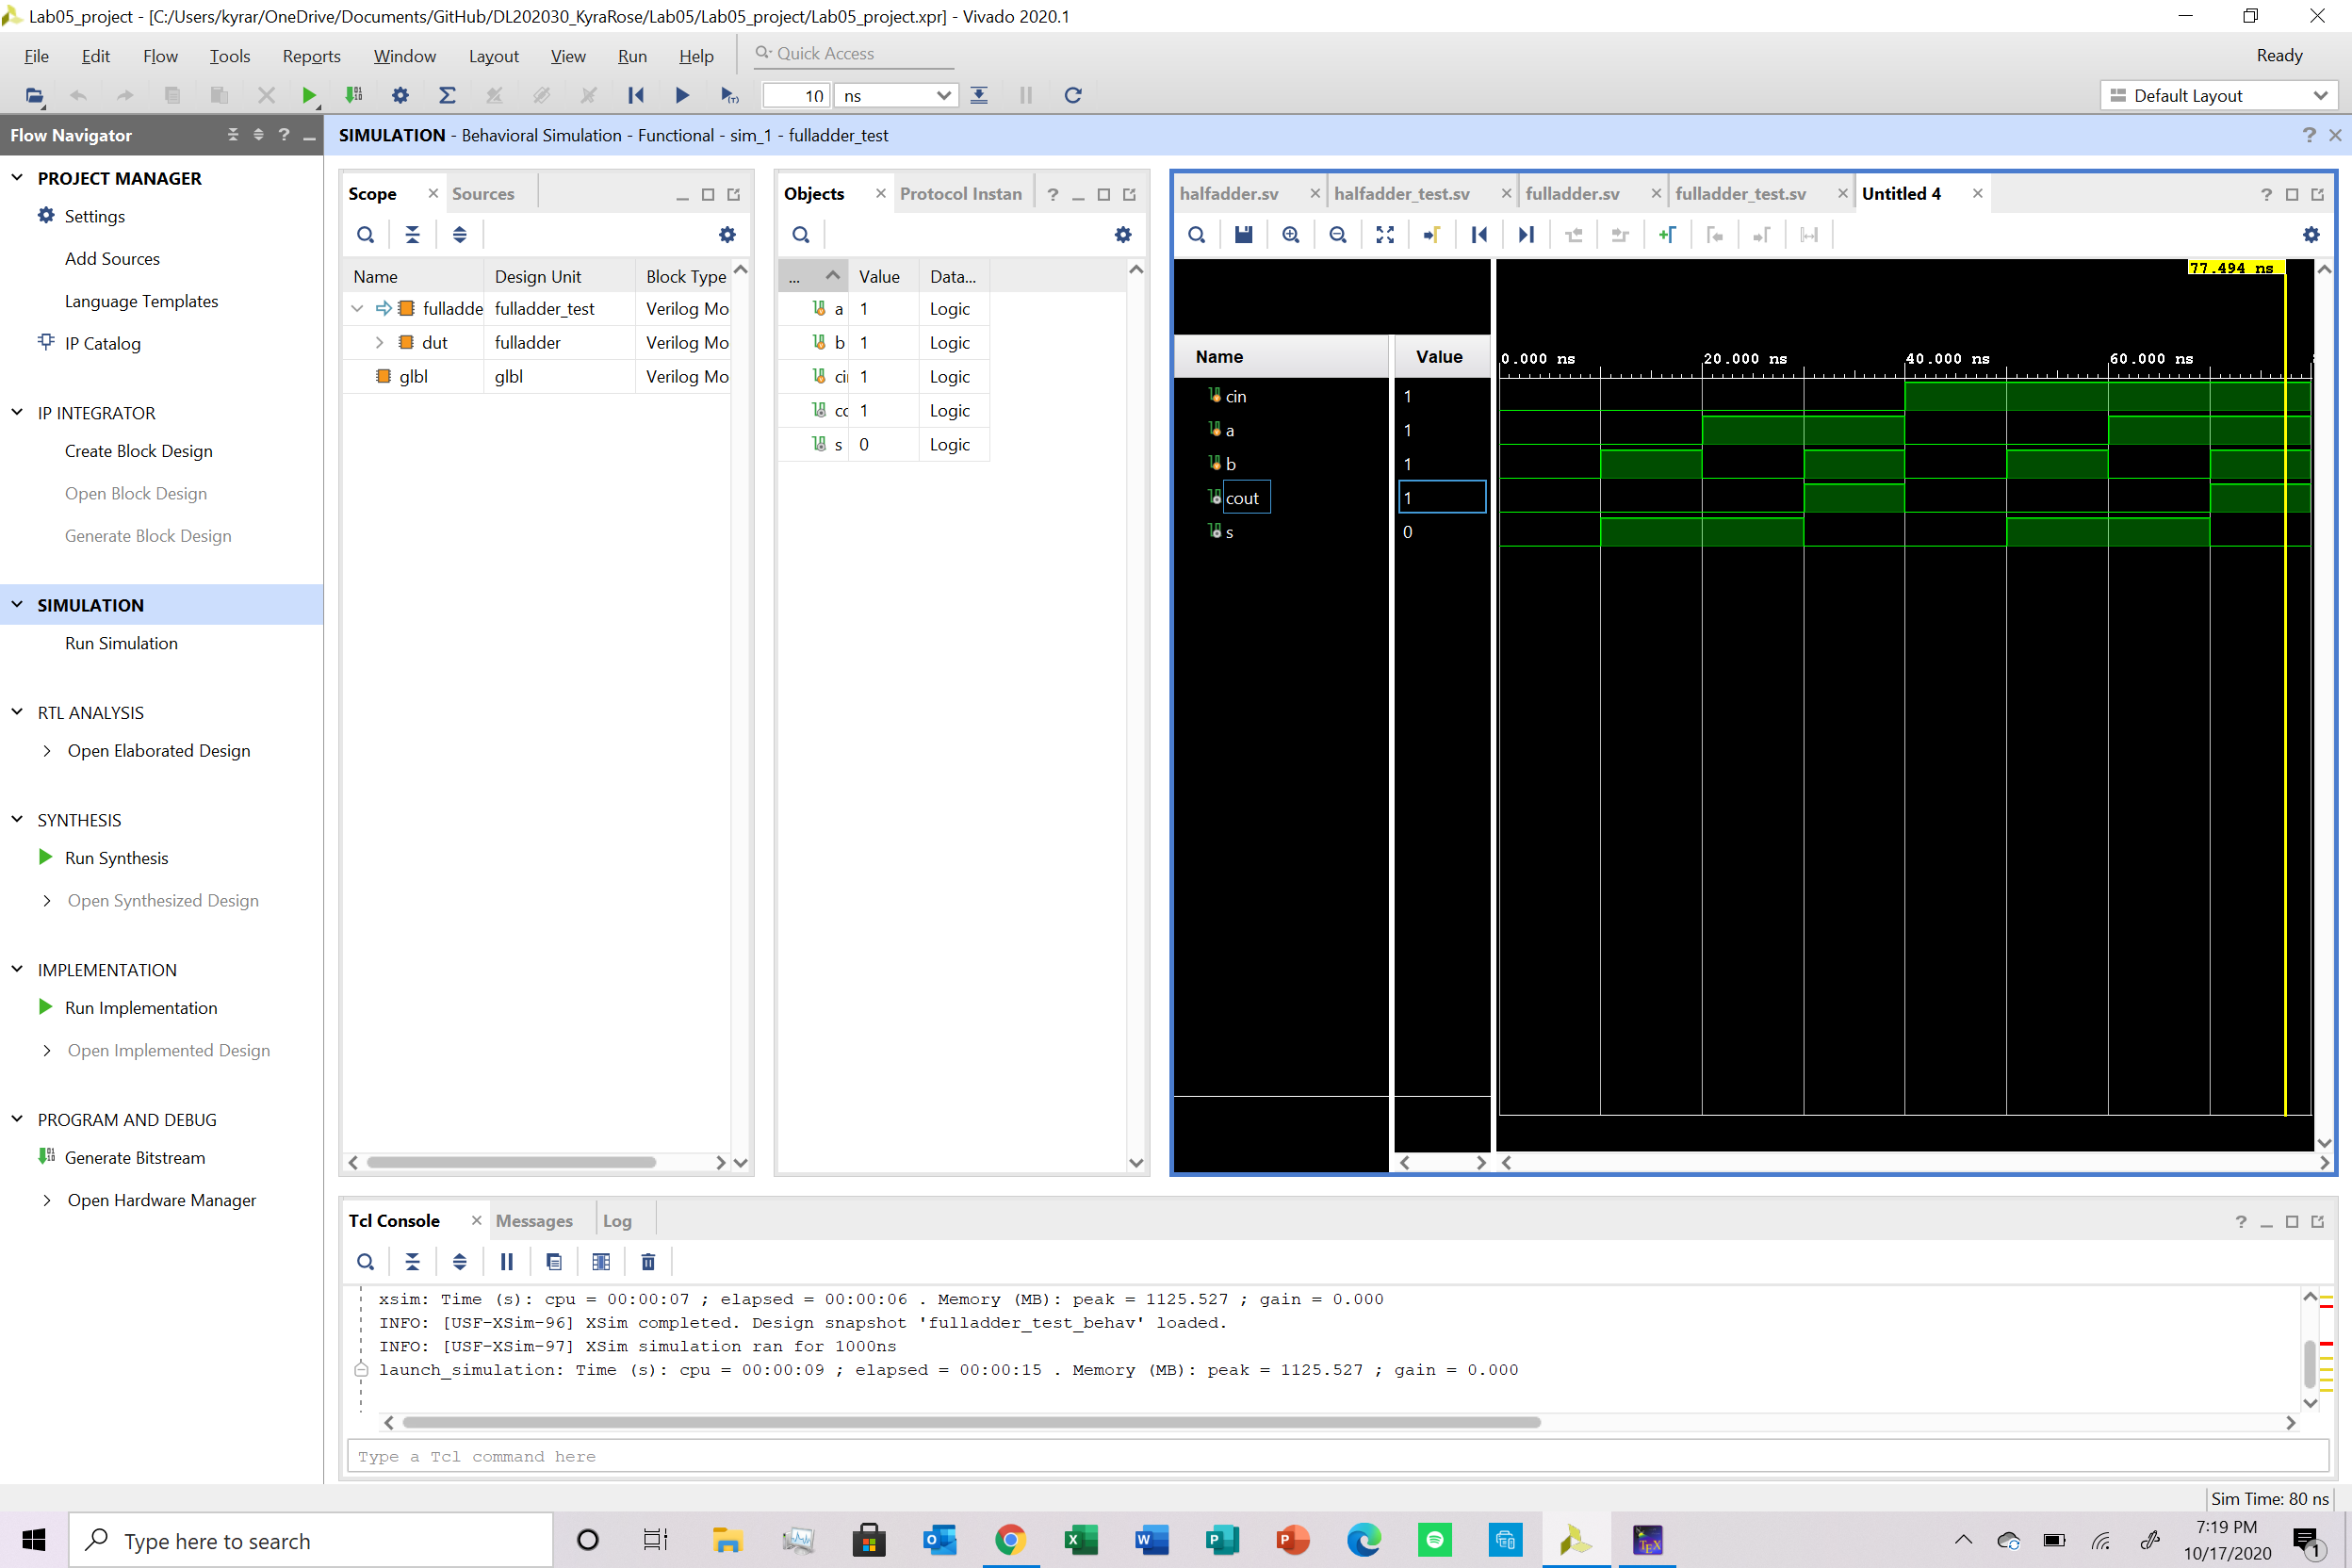
\includegraphics[width=0.5\textwidth,trim=43cm 30cm 0cm 8cm,clip]{fulladder sim}
	\caption{Full Adder Behavioral Simulation}
\end{figure}

\begin{figure}[h]\centering
	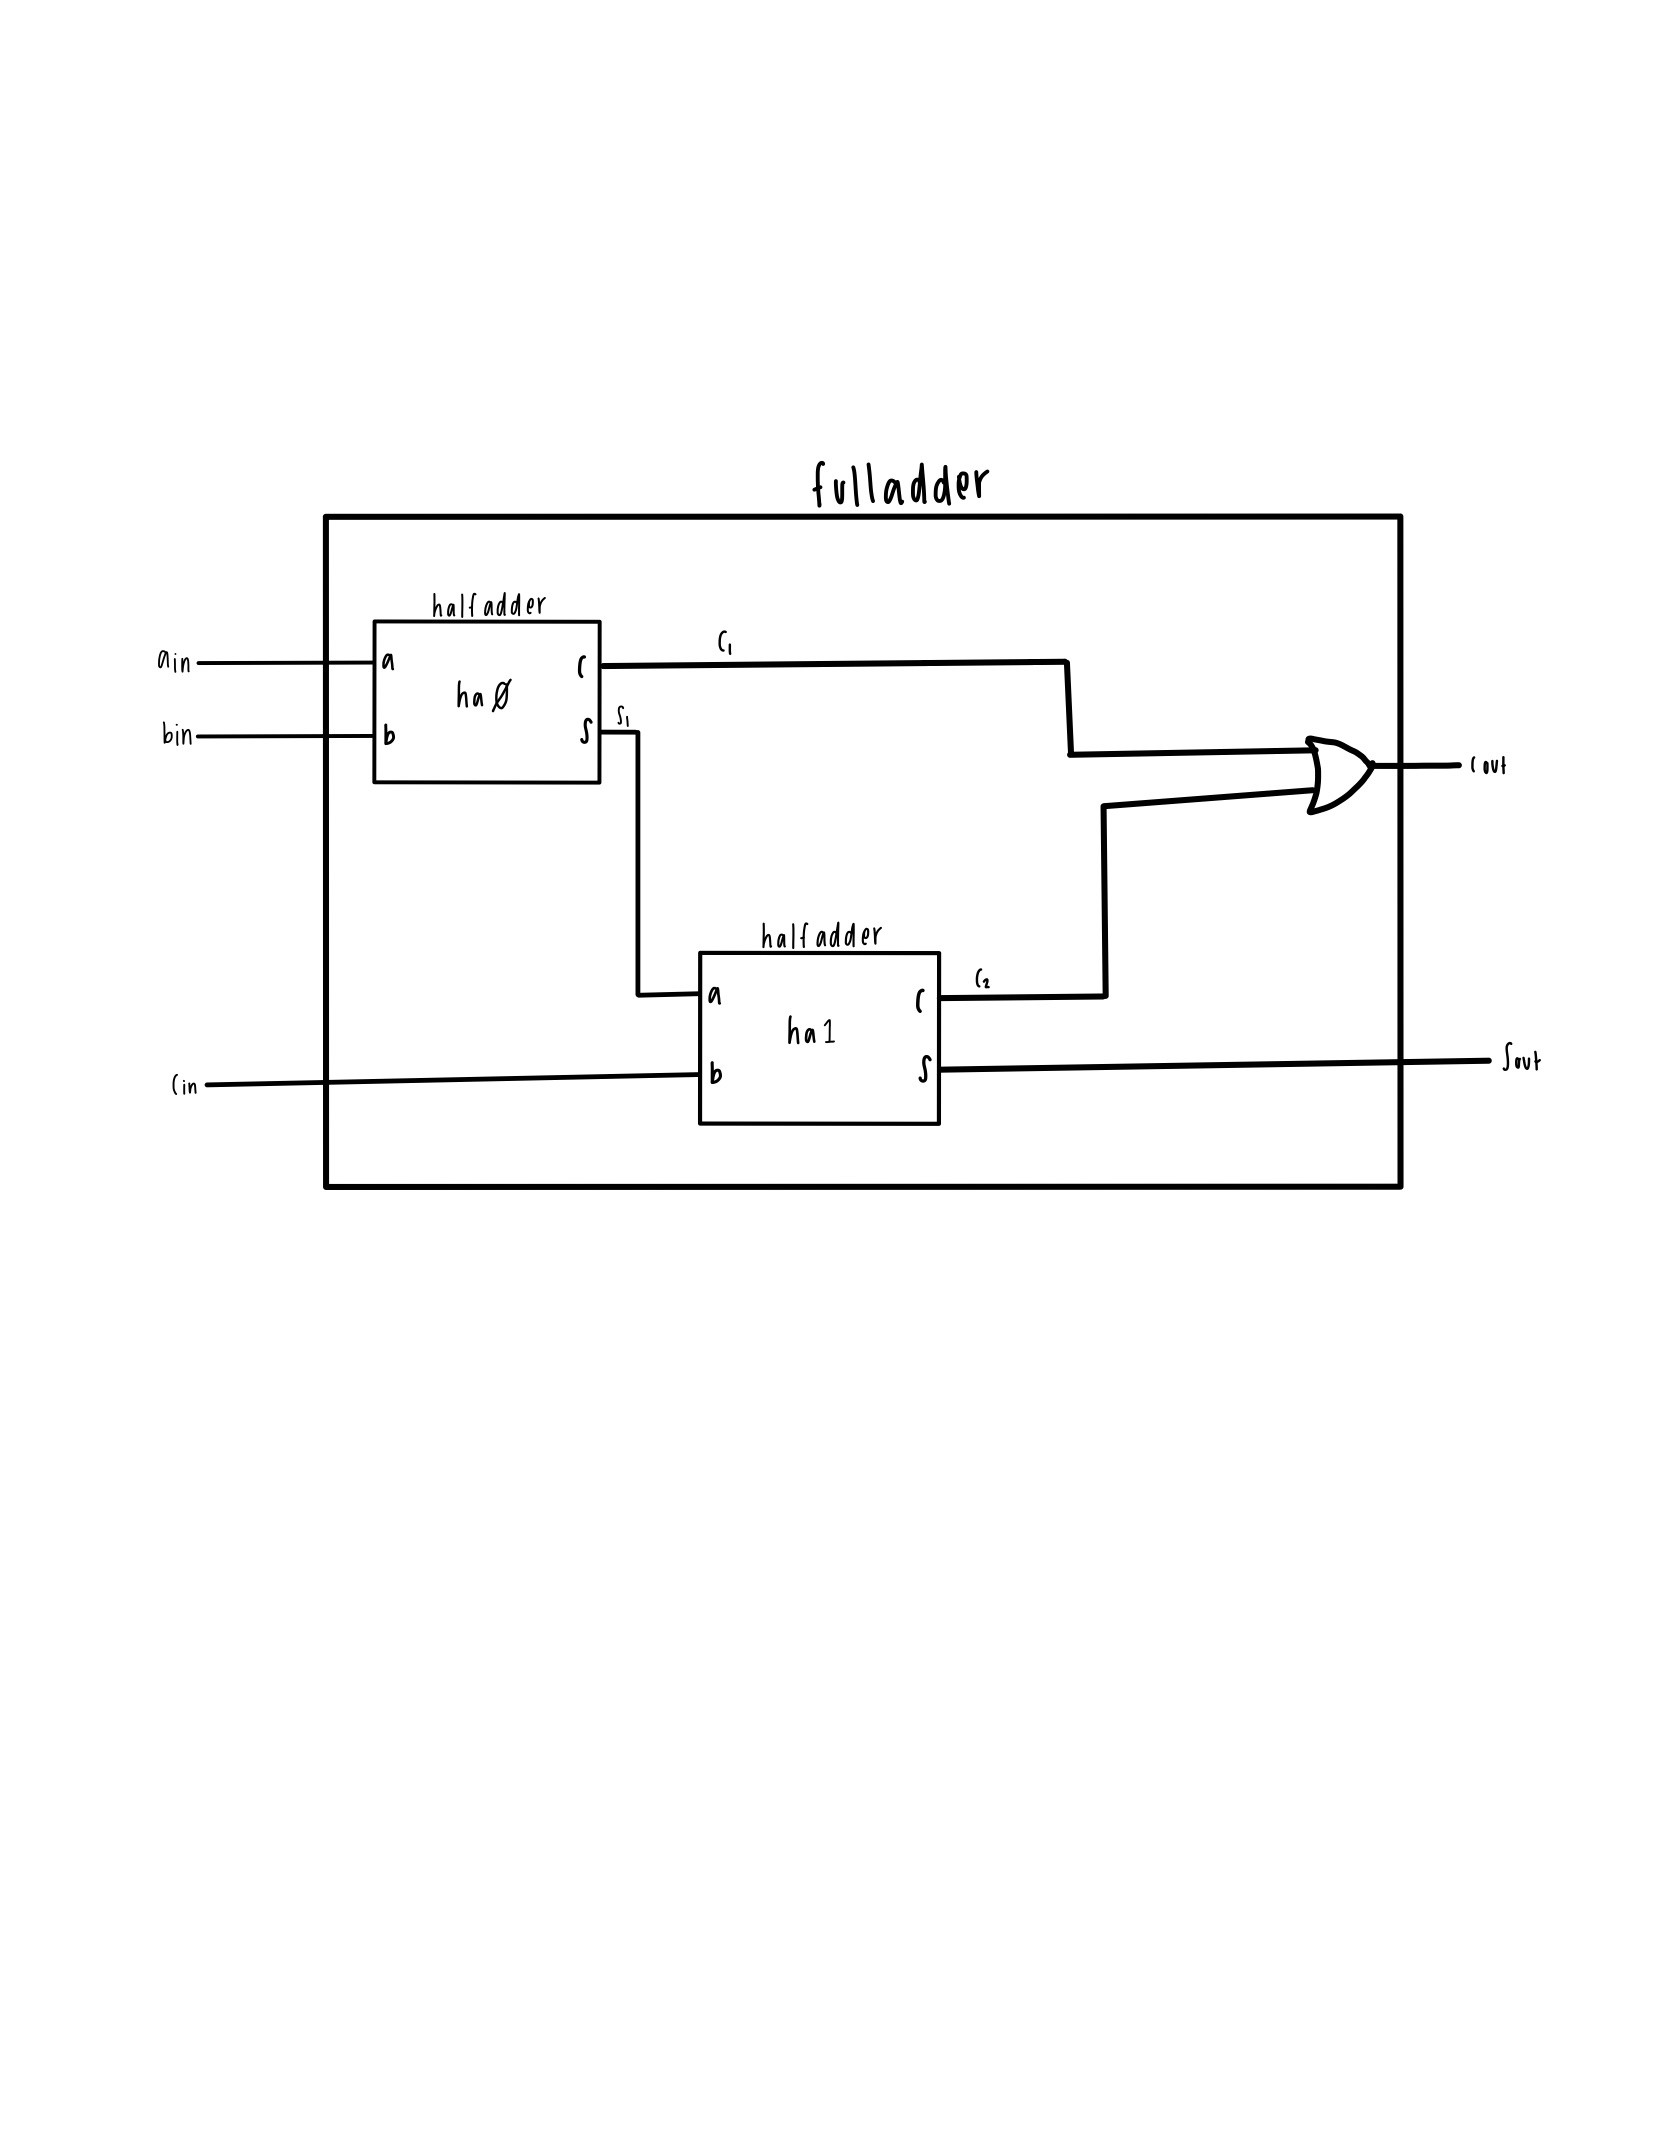
\includegraphics[width=0.5\textwidth,trim=0cm 25cm 0cm 10cm,clip]{fulladder block diagram}
	\caption{Full Adder Block Diagram}
\end{figure}

\begin{table}[h]\centering
	\caption{Adder Subtracter Truth Table }
	\label{tbl:example_table}
	\begin{tabular}{cc|ccc|c}
		\toprule
		A & B & B 2's comp & Sub (expected) & Dec & Sub (actual) \\
		\midrule
		00 & 01 & 111 & 111 & -7 & 011 \\
		00 & 10 & 110 & 110 & -6 & 010 \\
		00 & 11 & 101 & 101 & -5 & 001 \\
		01 & 01 & 111 & 000 & 0 & 100  \\
		10 & 01 & 111 & 001 & 1 & 101  \\
		10 & 00 & 000 & 010 & 2 & 110  \\
		\bottomrule
	\end{tabular} 
\end{table}

\begin{figure}[h]\centering
	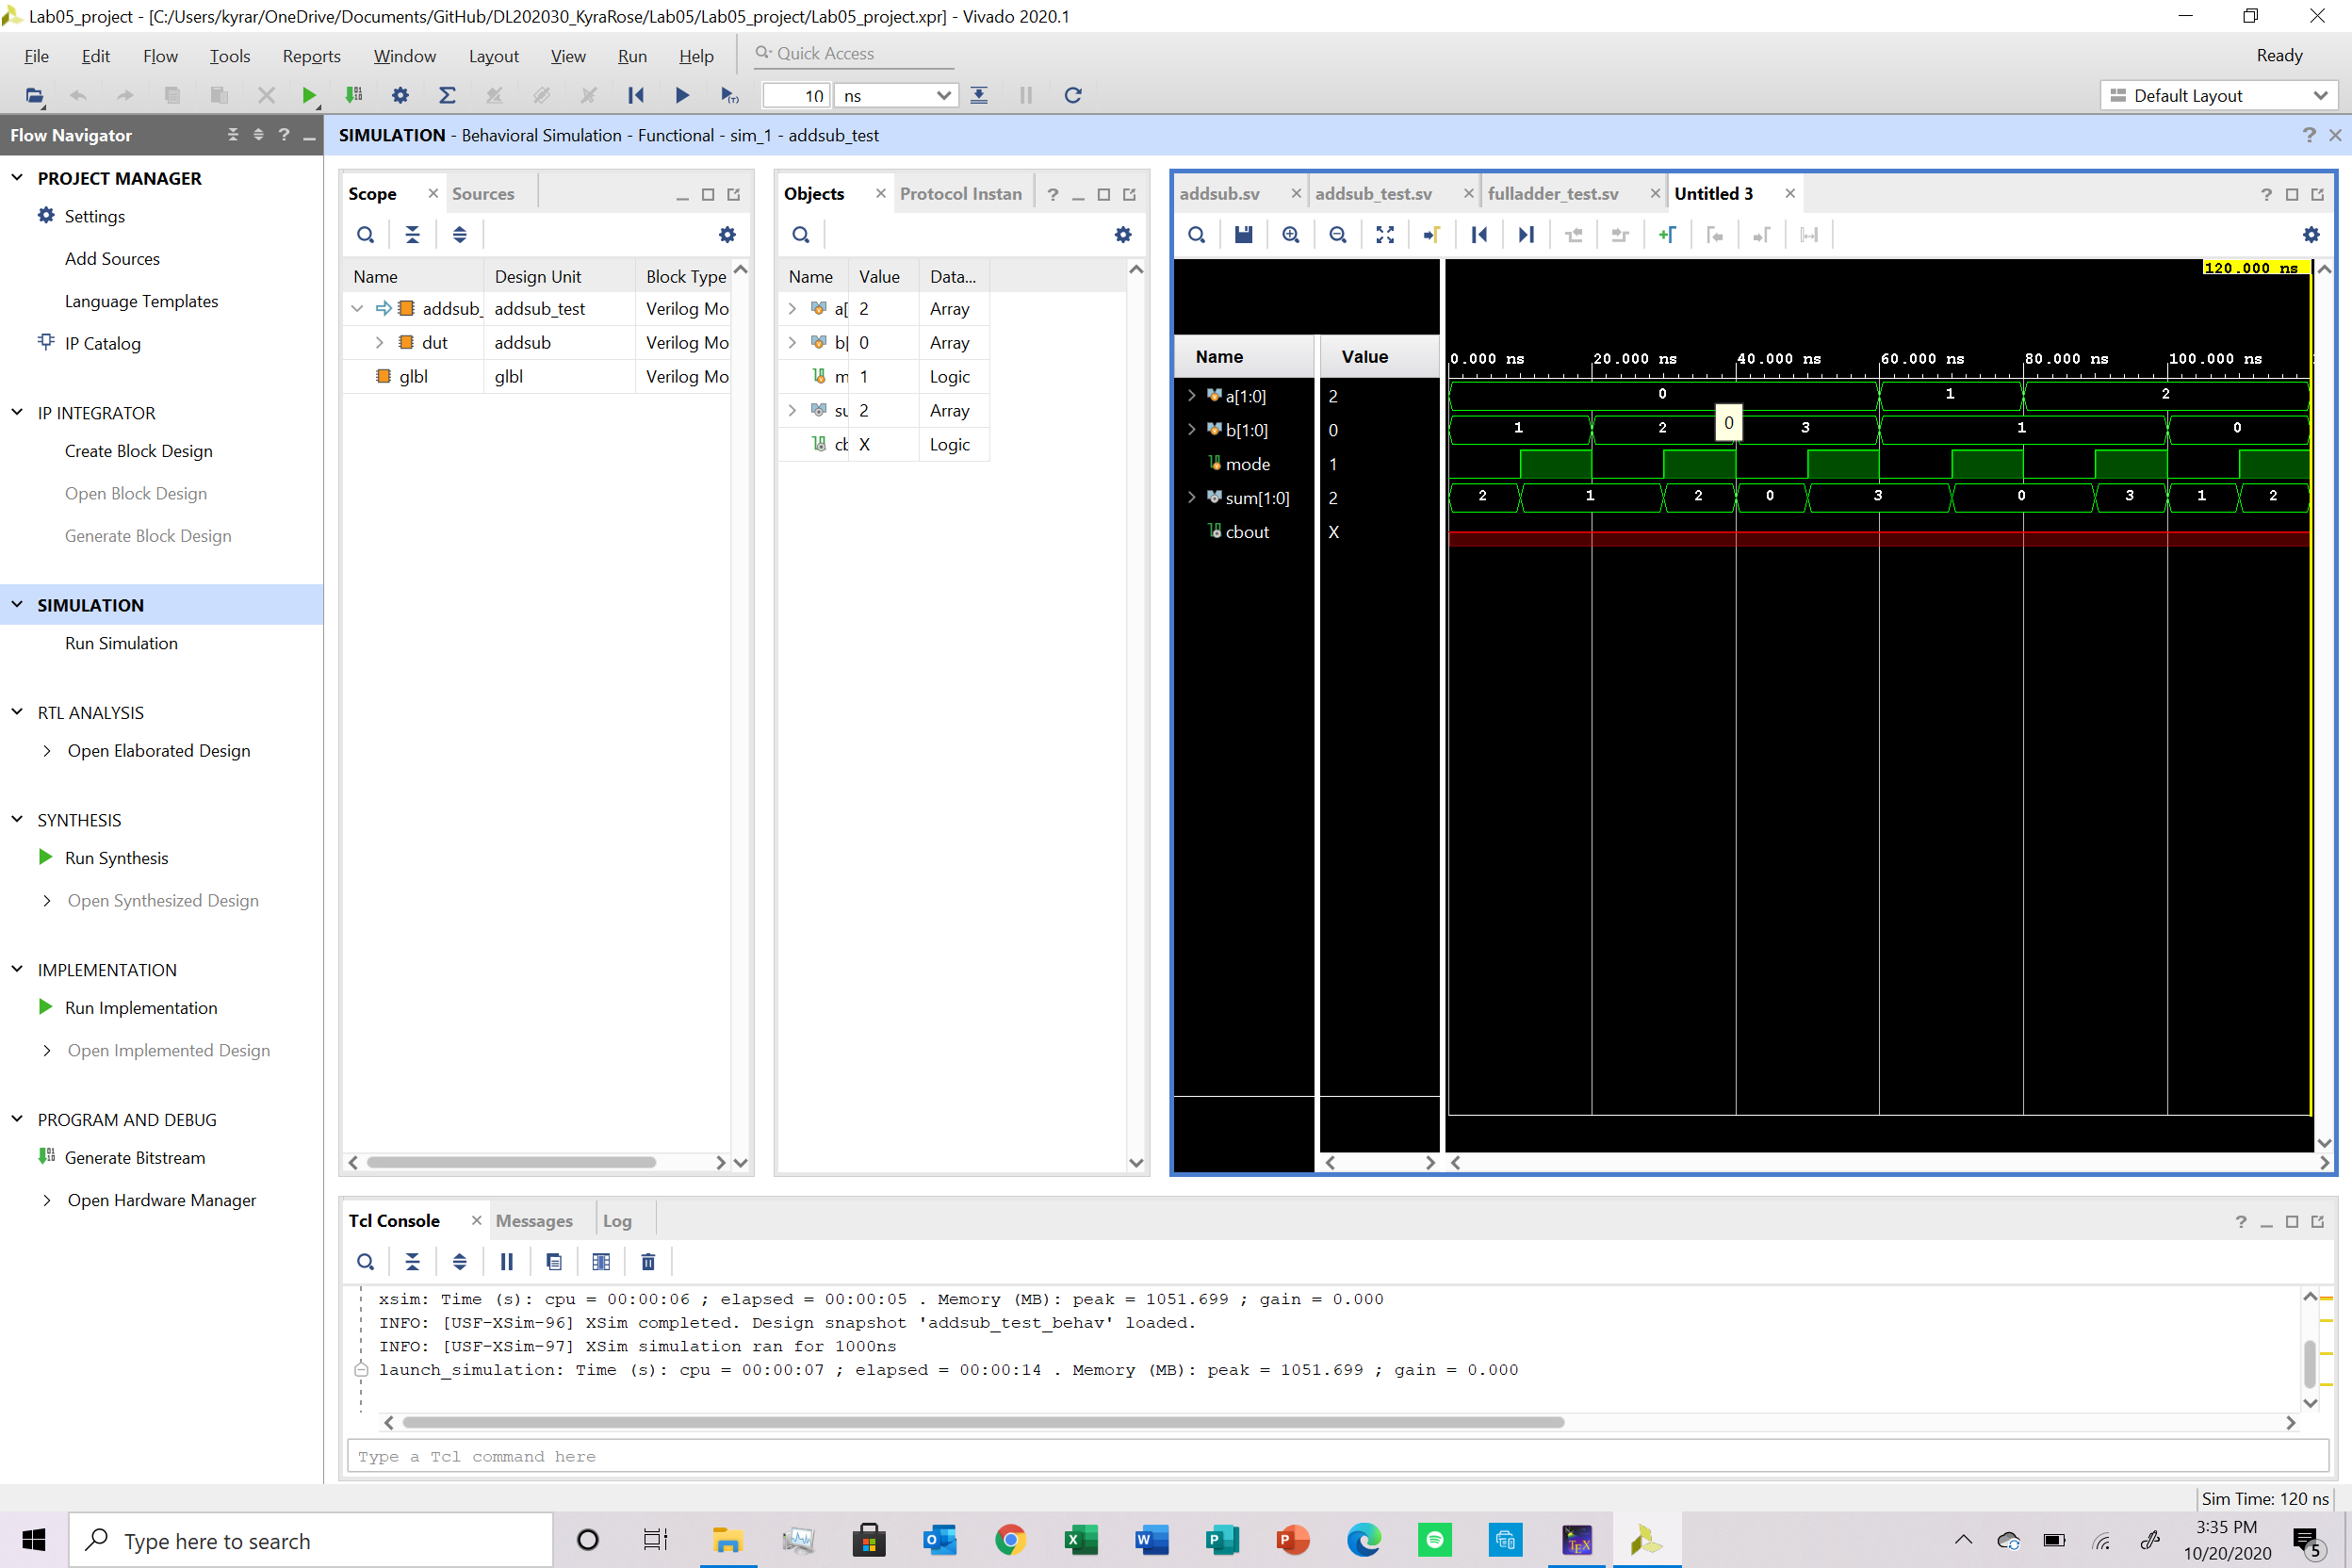
\includegraphics[width=0.5\textwidth,trim=43cm 30cm 0cm 8cm,clip]{addsub sim}
	\caption{Adder Subtractor Behavioral Simulation}
\end{figure}

\begin{figure}[h]\centering
	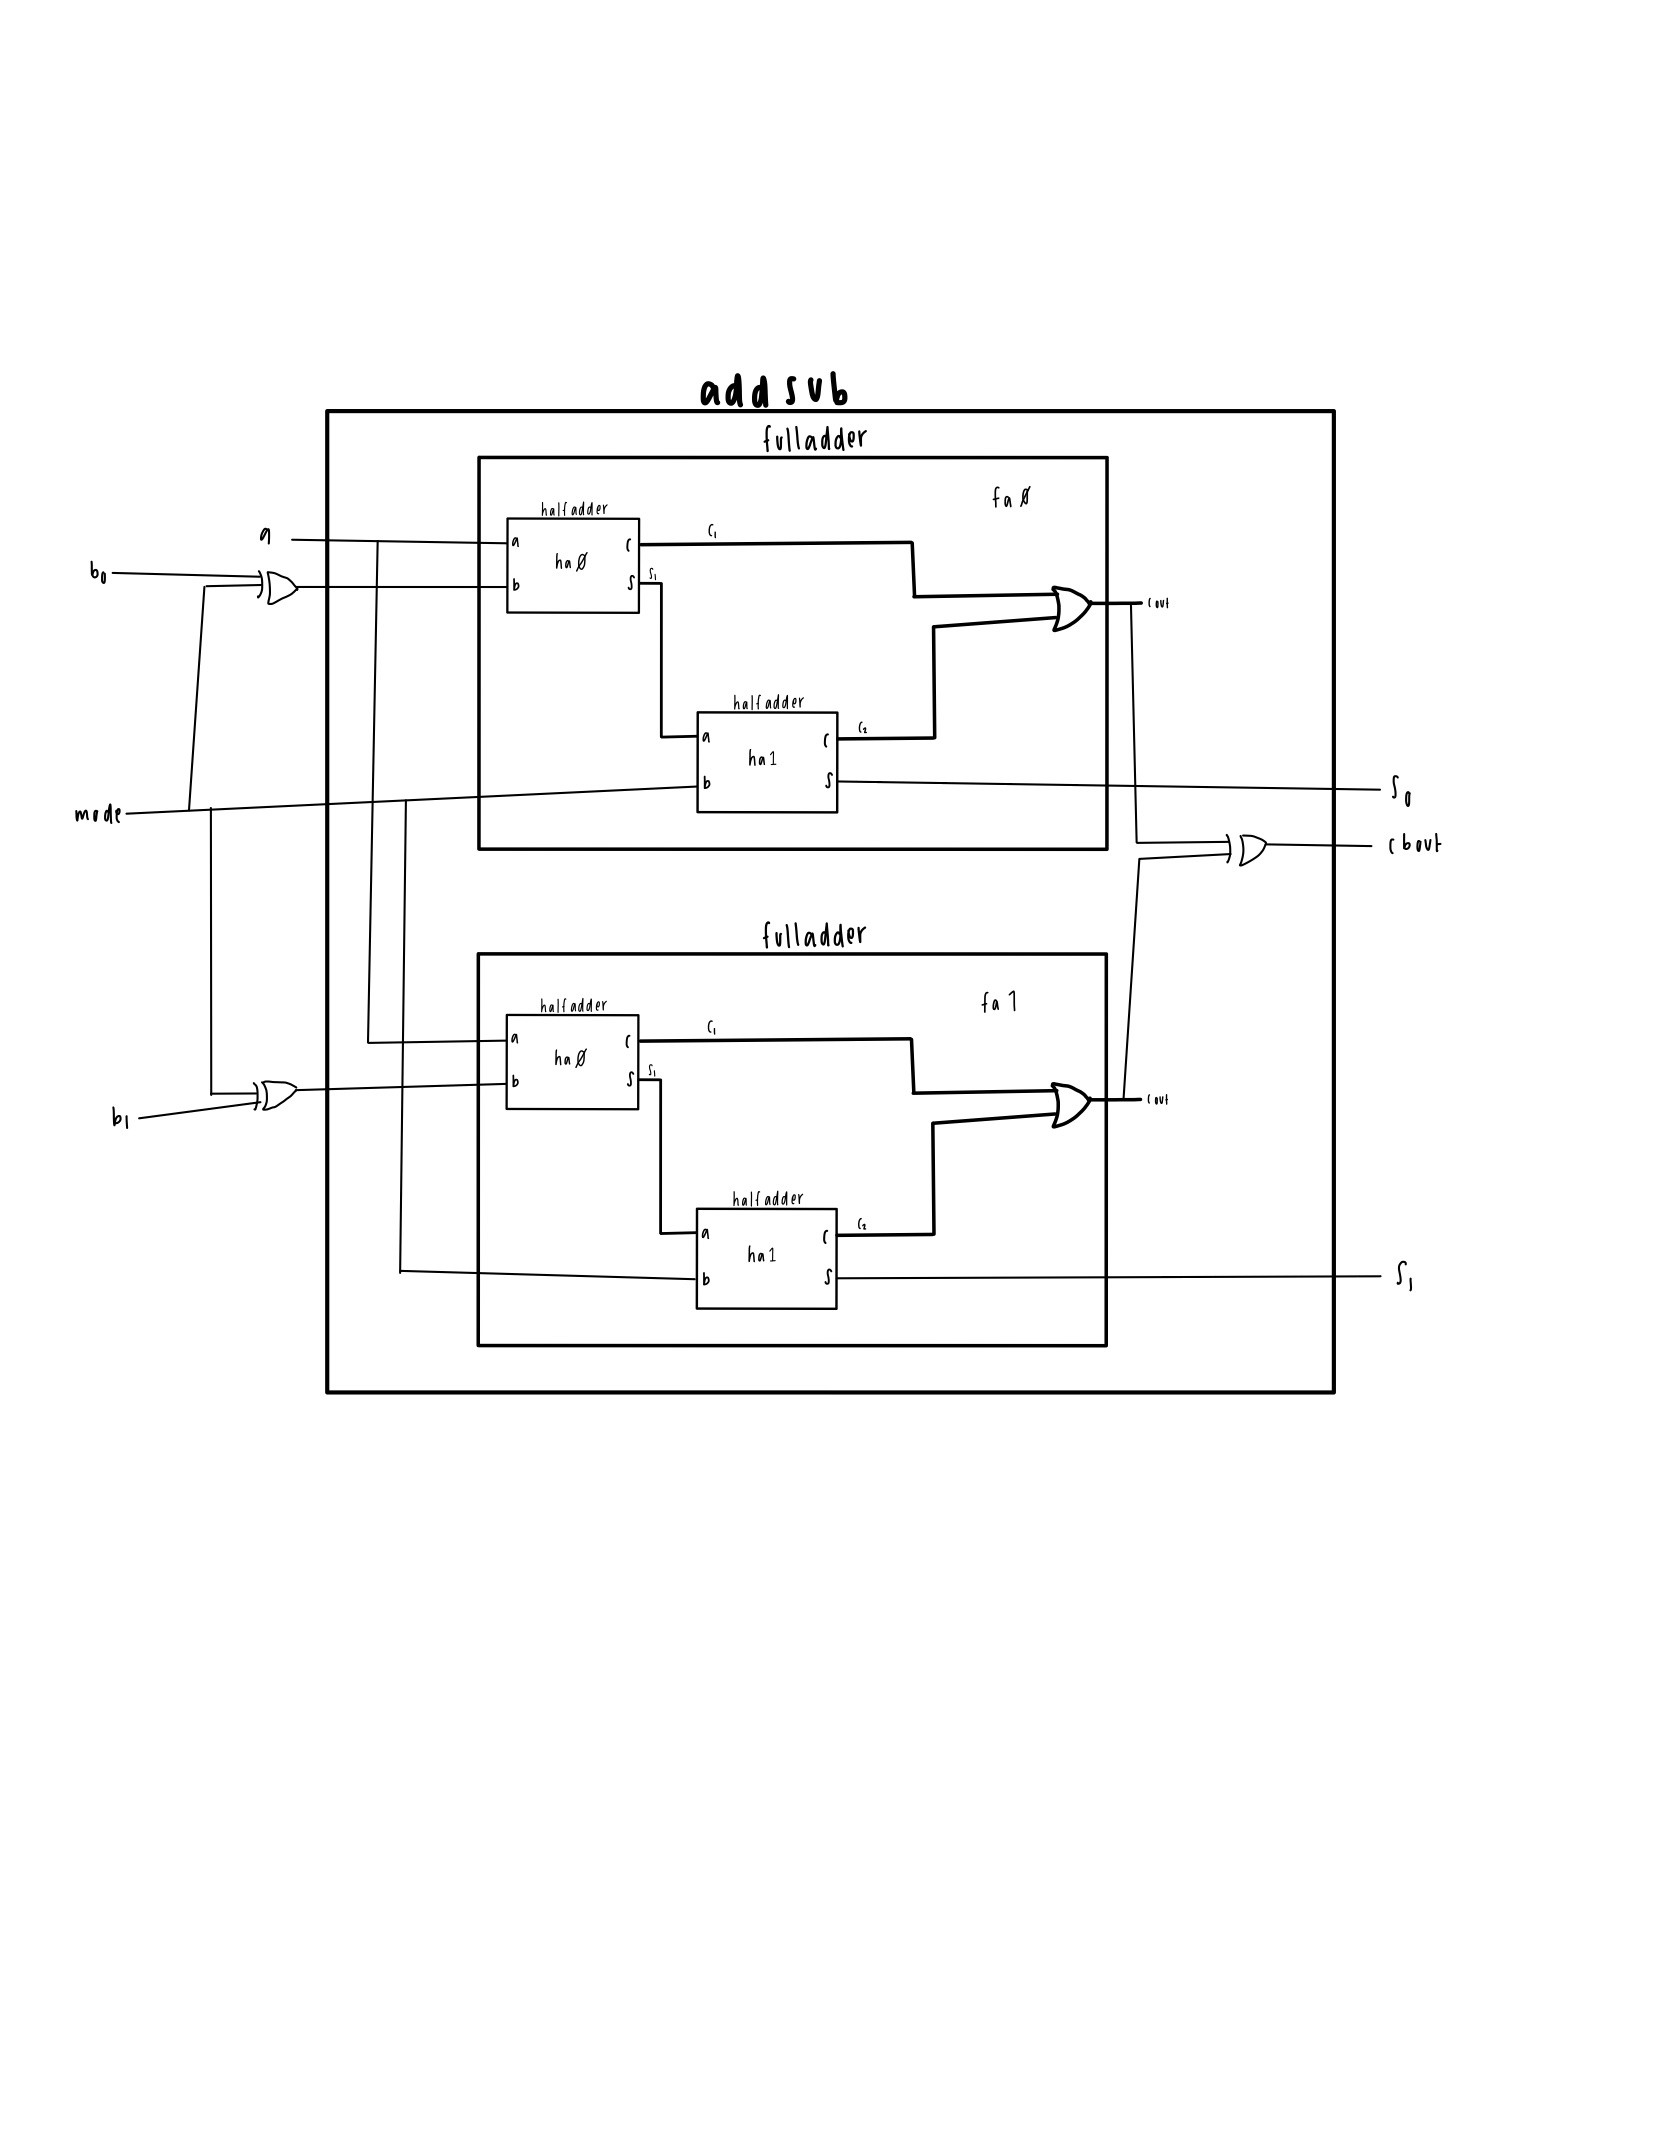
\includegraphics[width=0.5\textwidth,trim=0cm 20cm 0cm 10cm,clip]{addsub block diagram}
	\caption{Adder Subtractor Block Diagram}
\end{figure}


\end{document}
